\subsection{CNN Arithmetic and Parameter Counting}\label{sec:cnn-arithmetic-and-parameter-counting}

\subsubsection{One Input Channel and One Filter}\label{sec:one-input-channel-and-one-filter}

Until now, we focused on \textbf{how a convolutional layer works}. Now, the focus changes to: \textbf{given a convolutional layer, \emph{how do we compute the dimensions of its output and how many parameters does it contain?}} Let's start with the simplest case: a convolutional layer with \textbf{one input channel and one filter}. Suppose we have a convolutional layer with one input channel:
\begin{equation*}
    \text{Input: } 32 \times 32 \times 1 \quad \text{and} \quad \text{Filter: } 3 \times 3 \times 1
\end{equation*}
Nothing changes compared with the previous section: \textbf{one filter still produces one output map}. The only simplification is that  there is now only one input channel, so there is no summation over multiple channels $k$.

\highspace
\textcolor{Green3}{\faIcon{question-circle} \textbf{Now, if the input is $N \times N$, what is the size of the output?}} Until now we mostly discussed \emph{what} convolution computes. Now we begin asking: \emph{\textbf{how large is the result?}} Suppose the input is $5 \times 5$ and the kernel filter is $3 \times 3$. The filter cannot be centered on every input pixel, because near the borders, part of the filter would fall outside the image:

\begin{figure}[!htp]
    \centering
    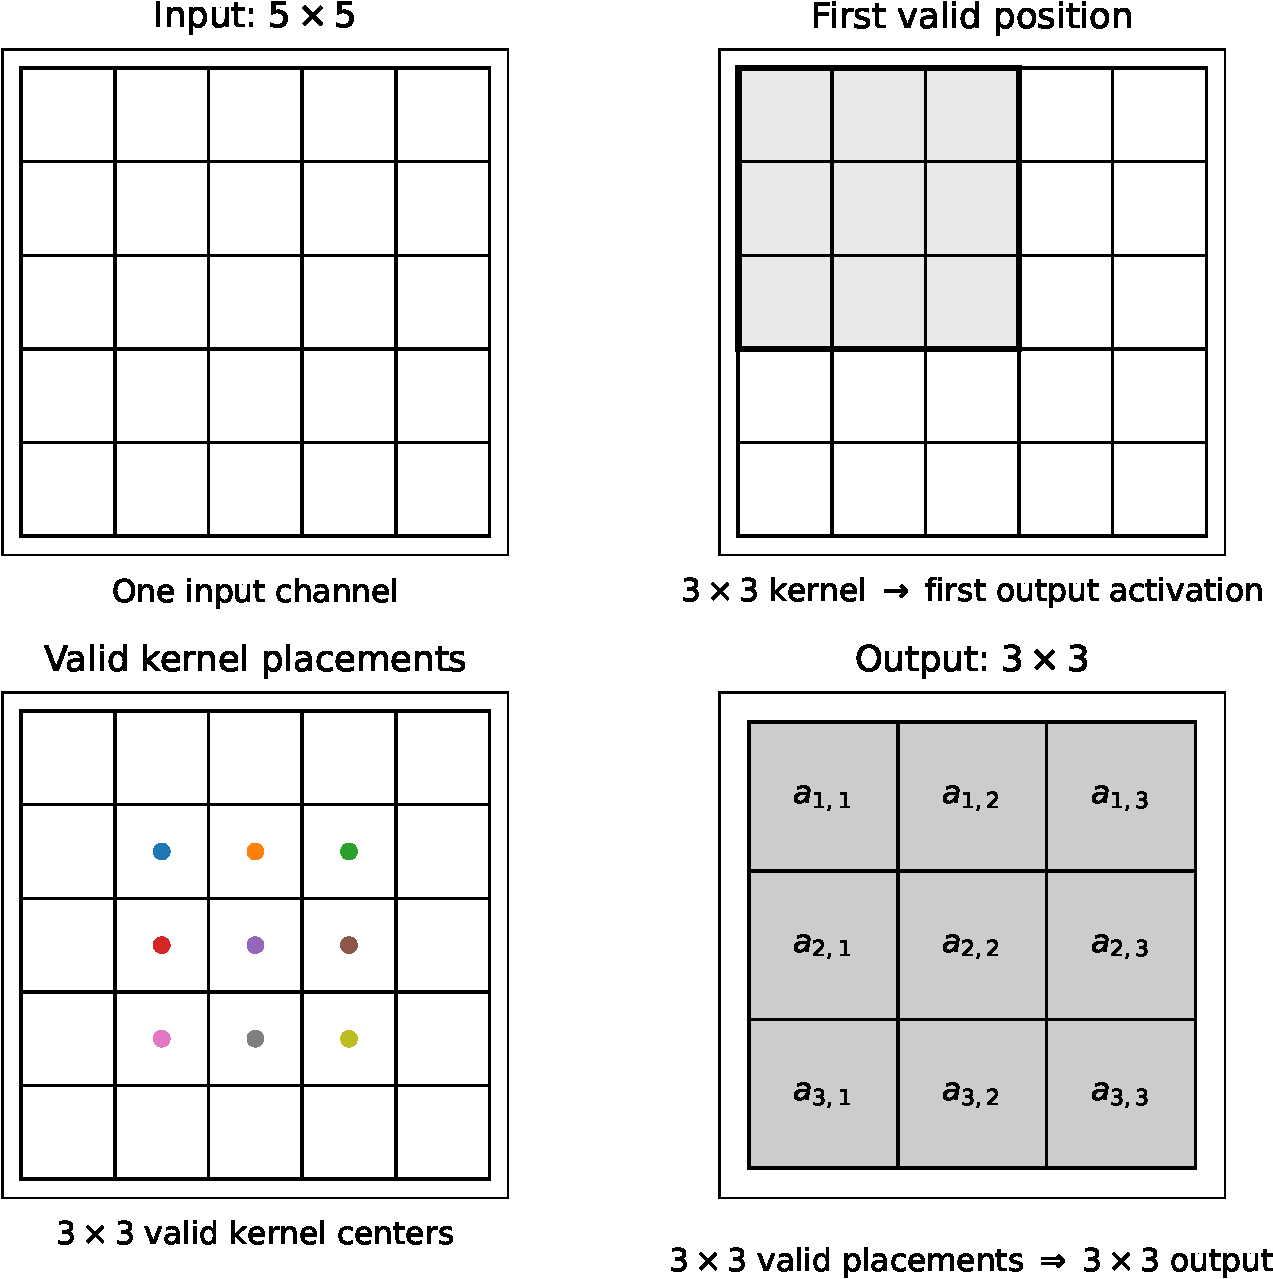
\includegraphics[width=\textwidth]{img/cnn/cnn_move_conv.pdf}
\end{figure}

\noindent
Considering the previous figure. If the input is $5 \times 5$, and the kernel is $3 \times 3$, with a stride (i.e., step size) of 1 and no padding (\autopageref{sec:padding}), the filter can occupy only $3 \times 3$ different positions. Therefore, the output will be $3 \times 3 \times 1$.

\highspace
In this section, we address the question, \emph{why and when does the spatial size shrink?}. The answer is that the \textbf{filter must remain entirely within the image}.

\highspace
However, this reasoning raises an issue. Without padding, the output is smaller than the input because the filter must remain entirely within the image. \emph{How can we fix this?} First, \emph{what happens when we add more filters and input channels?} \emph{How many parameters do we get?} \emph{Is there an equation to compute the output size?} We will answer these questions in the next sections.